%%%%%%%%%%%%%%%%%%%%%%%%%%%%%%%%%%%%%%%%%%%%%%%%%%
%%%%% General setting %%%%%
%%%%%%%%%%%%%%%%%%%%%%%%%%%%%%%%%%%%%%%%%%%%%%%%%%
\documentclass[t]{beamer}
\usecolortheme{default}
\usetheme{default}

%% Vietnamese %%
% \usepackage[utf8]{vietnam}
%%%%%%%%%%%%%%%%%%%%%%%%%%%%%%%%%%%%%%%%%%%%%%%%%%



%%%%%%%%%%%%%%%%%%%%%%%%%%%%%%%%%%%%%%%%%%%%%%%%%%
%%%%% Tikz %%%%%
%%%%%%%%%%%%%%%%%%%%%%%%%%%%%%%%%%%%%%%%%%%%%%%%%%
\usepackage{pgfplots} %%%%%% Regression %%%%
\pgfplotsset{compat = newest}
\usepackage{pgfplotstable}
\usepackage{tikz}
\usepackage{tikz-3dplot} %%%%%% Draw %%%%%%
\usepackage{tikz,tkz-euclide}
\usetikzlibrary{arrows,calc,patterns}
% \usetikzlibrary{quotes,angles}
%\usetikzlibrary{shapes.geometric}
\usepackage{circuitikz} %%%%% Circuit %%%%
%\usetikzlibrary{decorations.pathmorphing,patterns}

%%%%%%%%%%%%%%%%%%%%%%%%%%%%%%%%%%%%%%%%%%%%%%%%%%

%% Color %%
\definecolor{BlueDefault}{rgb}{0.2,0.2,0.7}


%%%%%%%%%%%%%%%%%%%%%%%%%%%%%%%%%%%%%%%%%%%%%%%%%%
%%%%% Figure and Table %%%%%
%%%%%%%%%%%%%%%%%%%%%%%%%%%%%%%%%%%%%%%%%%%%%%%%%%

\usepackage{graphicx} % Required for inserting images

%% Caption of Figure and Table %%
\usepackage{caption}
% \captionsetup[figure]{labelsep=space,justification=centering}
% \captionsetup[table]{labelsep=space,justification=centering}

% Column, Row and Minipage %%
% \usepackage{minipage}

%%%%%%%%%%%%%%%%%%%%%%%%%%%%%%%%%%%%%%%%%%%%%%%%%%


%%%%%%%%%%%%%%%%%%%%%%%%%%%%%%%%%%%%%%%%%%%%%%%%%%
%%%%% General Information %%%%%
%%%%%%%%%%%%%%%%%%%%%%%%%%%%%%%%%%%%%%%%%%%%%%%%%%
\title{Metamaterials}
\author{Nguyen Thanh Long}
\institute{RF3i - Smart Sensor Lab}
% \date{\today}
\date{}
%%%%%%%%%%%%%%%%%%%%%%%%%%%%%%%%%%%%%%%%%%%%%%%%%%

%% Make Table of Contents %%
\AtBeginSection[]{
  \begin{frame}
  \frametitle{Outline}
  \tableofcontents[currentsection]
  \end{frame}
}

%% Section numbering %%
\setbeamertemplate{section in toc}[sections numbered]
\setbeamertemplate{subsection in toc}[subsections numbered]


%%%%%%%%%%%%%%%%%%%%%%%%%%%%%%%%%%%%%%%%%%%%%%%%%%
%%%%% Headline & Footline %%%%%
%%%%%%%%%%%%%%%%%%%%%%%%%%%%%%%%%%%%%%%%%%%%%%%%%%

%% Make page number %%
\setbeamertemplate{footline}[page number]

%% Headline %%
\setbeamertemplate{headline}
{
    \begin{beamercolorbox}{section in head/foot}
    % \vskip2pt\insertnavigation{\paperwidth}\vskip2pt
    \vskip2pt\insertsectionnavigationhorizontal{.5\textwidth}{\hskip0pt plus1filll}{}\vskip2pt
    
    \end{beamercolorbox}
}

%% Footline %%
\setbeamertemplate{footline}
{
    \hbox{%
  
    \begin{beamercolorbox}[wd=.333333\paperwidth,ht=2.25ex,dp=1ex,center]{author in head/foot}%
        \usebeamerfont{author in head/foot}\insertshortauthor
    \end{beamercolorbox}%
  
    \begin{beamercolorbox}[wd=.333333\paperwidth,ht=2.25ex,dp=1ex,center]{title in head/foot}%
        \usebeamerfont{title in head/foot}\insertshorttitle
    \end{beamercolorbox}%
  
    \begin{beamercolorbox}[wd=.333333\paperwidth,ht=2.25ex,dp=1ex,right]{date in head/foot}%
        \usebeamerfont{date in head/foot}\insertshortdate{}\hspace*{2em}
        \usebeamerfont{page number in head/foot}\insertframenumber{} / \inserttotalframenumber\hspace*{2ex}
    \end{beamercolorbox}}%
  
    \vskip0pt%
}
%%%%%%%%%%%%%%%%%%%%%%%%%%%%%%%%%%%%%%%%%%%%%%%%%%

%%%%%%%%%%%%%%%%%%%%%%%%%%%%%%%%%%%%%%%%%%%%%%%%%%
%%%%% Mathematics %%%%%
%%%%%%%%%%%%%%%%%%%%%%%%%%%%%%%%%%%%%%%%%%%%%%%%%%
\usepackage{esint} % various fancy integral symbols
\usepackage{bm} % bf vector
\usepackage{siunitx}
%%%%%%%%%%%%%%%%%%%%%%%%%%%%%%%%%%%%%%%%%%%%%%%%%%

%%%%%%%%%%%%%%%%%%%%%%%%%%%%%%%%%%%%%%%%%%%%%%%%%%
%%%%% Biblioraphy %%%%%
%%%%%%%%%%%%%%%%%%%%%%%%%%%%%%%%%%%%%%%%%%%%%%%%%%
\usepackage[backend=biber,style=ieee]{biblatex}
\addbibresource{Metamaterials.bib}

\usepackage{url}
\usepackage{hyperref}
\hypersetup{
	colorlinks=true,
	linkcolor=black,
	filecolor=blue,
    citecolor=purple,
	urlcolor=blue,
	pdftitle={Overleaf Example},
	pdfpagemode=FullScreen,
}
%%%%%%%%%%%%%%%%%%%%%%%%%%%%%%%%%%%%%%%%%%%%%%%%%%


\begin{document}

% \maketitle
\frame{\titlepage}

\section{Introduction to metamaterials}

\subsection{What is metamaterial}

\begin{frame}{What is metamaterial?}
    \begin{columns}
        \column{0.5\textwidth}
        Metamaterials:
        \begin{itemize}
            \item Properties depend on structure.
            \item Usually based on periodic structure.
        \end{itemize}
        \vspace{1mm}
        Unusual properties and applications:
        \begin{itemize}
            \item Negative permittivity and permeability.
            \item Perfect absorber.
            \item Perfect lens.
            \item Bending waves.
            \item ...
        \end{itemize}
        \column{0.5\textwidth}
        \begin{figure}
            \centering
            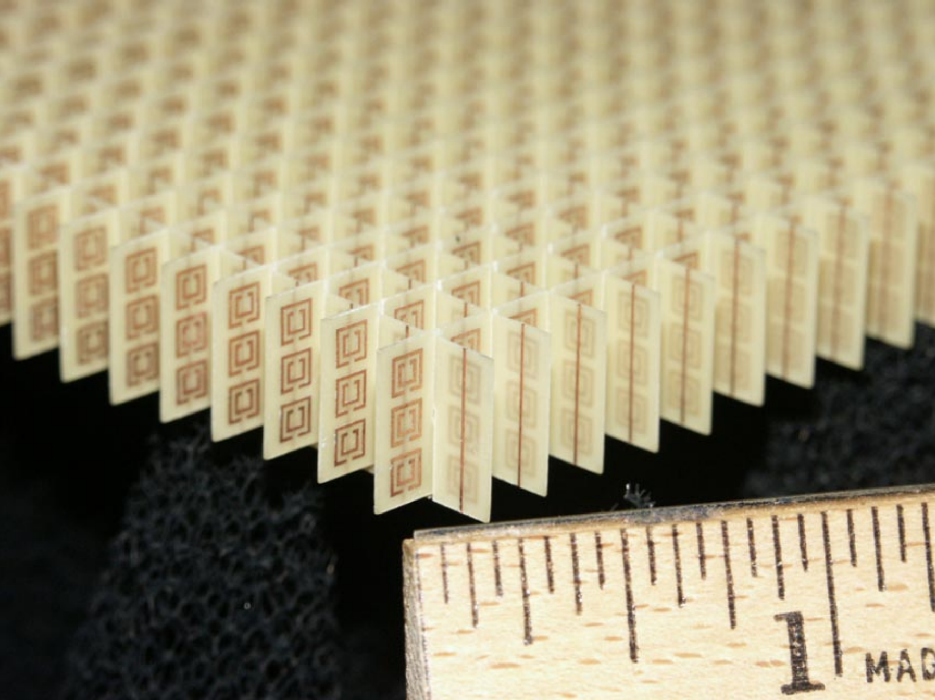
\includegraphics[width=\textwidth]{Figures/Meta_DN.pdf}
            \caption{Periodic structure. \cite{10.1063/1.1850590}}
            \label{fig:Periodic_structure}
        \end{figure}
    \end{columns}
\end{frame}

\subsection{Plasma oscillation}

\begin{frame}{Plasma oscillation}
    \begin{columns}
        \column{0.5\textwidth}
        
        \vspace{2mm}
        \begin{itemize}
            \item Permitivity:
        \end{itemize}
        \begin{equation*}
            \varepsilon (\omega) = \varepsilon_0 \left(1 -  \dfrac{\omega_P^2}{\omega^2 - j \gamma \omega } \right)
        \end{equation*}
        can be negative in low frequency, but the loss is very high.
        \vspace{5mm}
        \begin{itemize}
            \item Plasma frequency:
        \end{itemize}
        \begin{equation*}
            \omega_P^2 = \dfrac{ne^2}{\varepsilon_0 m}.
        \end{equation*}
        \column{0.5\textwidth}

        \begin{figure}
            \centering
            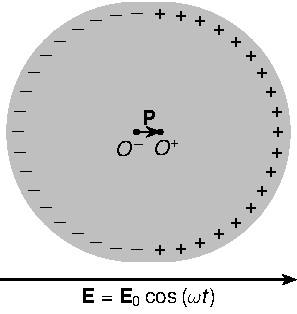
\includegraphics[width=\textwidth]{Figures/Rayleigh_scattering.pdf}
            \caption{Plasma oscillation}
            \label{fig:Plasma oscillation}
        \end{figure}
    \end{columns}
\end{frame}

\subsection{Transmission Line Model}

\begin{frame}{Transmission Line Model}
    \begin{figure}
        \centering
        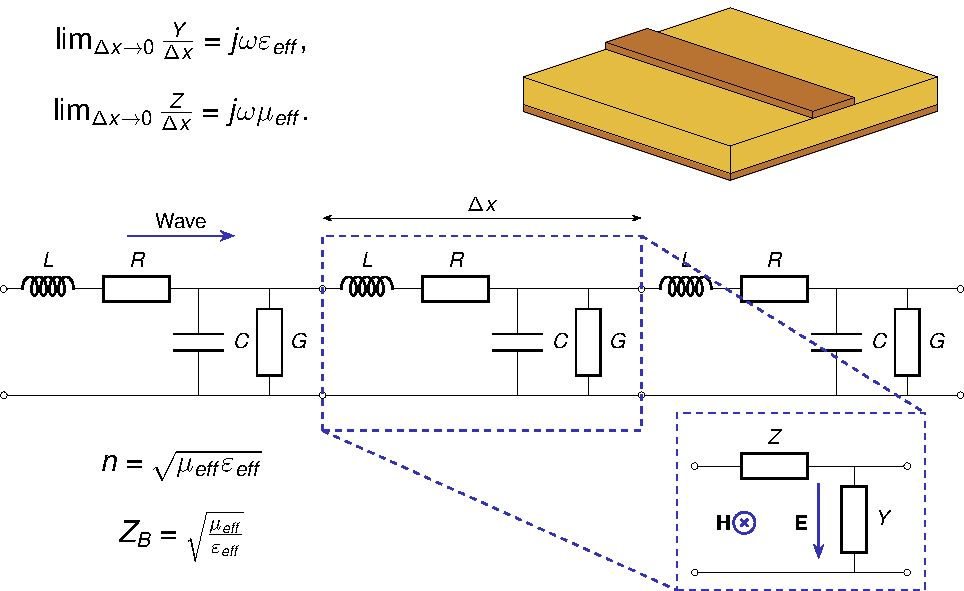
\includegraphics[width=\textwidth]{Figures/TL_equivalent_circuit.pdf}
        \caption{Transmission line model. \cite{maasch2016tunable}}
        \label{fig:TL_equivalent_circuit}
    \end{figure}
\end{frame}

\section{Invention of the metamaterial}

\subsection{Wire Lattice structure}

\begin{frame}{Wire Lattice structure}
    \begin{columns}
        \column{0.5\textwidth}
        \begin{itemize}
            \item Effective permittivity \cite{PhysRevLett.76.4773}:
        \end{itemize}
        \begin{equation*}
            \varepsilon (\omega) = \varepsilon_0 \left( 1 - \dfrac{\omega_{P \varepsilon}^2}{\omega^2 - j \gamma \omega } \right).
        \end{equation*}
        % \vspace{3mm}
        \begin{itemize}
            \item Plasma frequency
        \end{itemize}
        \begin{equation*}
            \omega_{P \varepsilon} = \sqrt{ \dfrac{2 \pi c_0^2}{a^2 \ln (a/R)} } \sim \dfrac{c_0}{a}.
        \end{equation*}
        \begin{itemize}
            \item Effective permittivity tensor:
        \end{itemize}
        \begin{equation*}
            \varepsilon_{eff} = \left(
            \begin{array}{ccc}
                \varepsilon_0 & 0 & 0 \\
                0 & \varepsilon_0 & 0 \\ 
                0 & 0 & \varepsilon (\omega)
            \end{array}
            \right) .
        \end{equation*}

        \column{0.5\textwidth}
        \vspace{-14mm}
        \begin{figure}
            \centering
            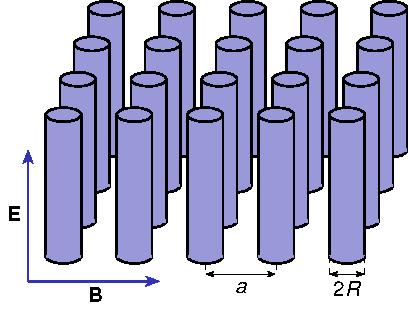
\includegraphics[width=0.8\textwidth]{Figures/Wire_lattice_structure.pdf}
            \caption{Wire lattice structure.}
            \label{fig:Wire_lattice_structure}
        \end{figure}
        \vspace{-8mm}
        \begin{figure}
            \centering
            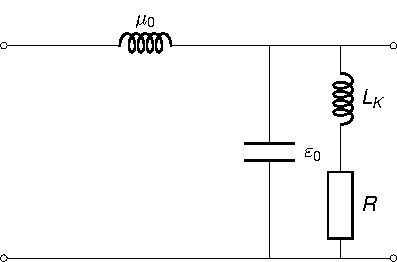
\includegraphics[width=0.8\textwidth]{Figures/TL_negative_permittivity.pdf}
            \caption{Equivalent circuit of wire lattice structure.}
            \label{fig:TL_negative_permittivity}
        \end{figure}
        
    \end{columns}
\end{frame}

\subsection{Split-Ring Resonator structure}

\begin{frame}{Split-Ring Resonator structure}
    \begin{columns}
        \column{0.6\textwidth}
        \cite{798002}
        \begin{figure}
            \centering
            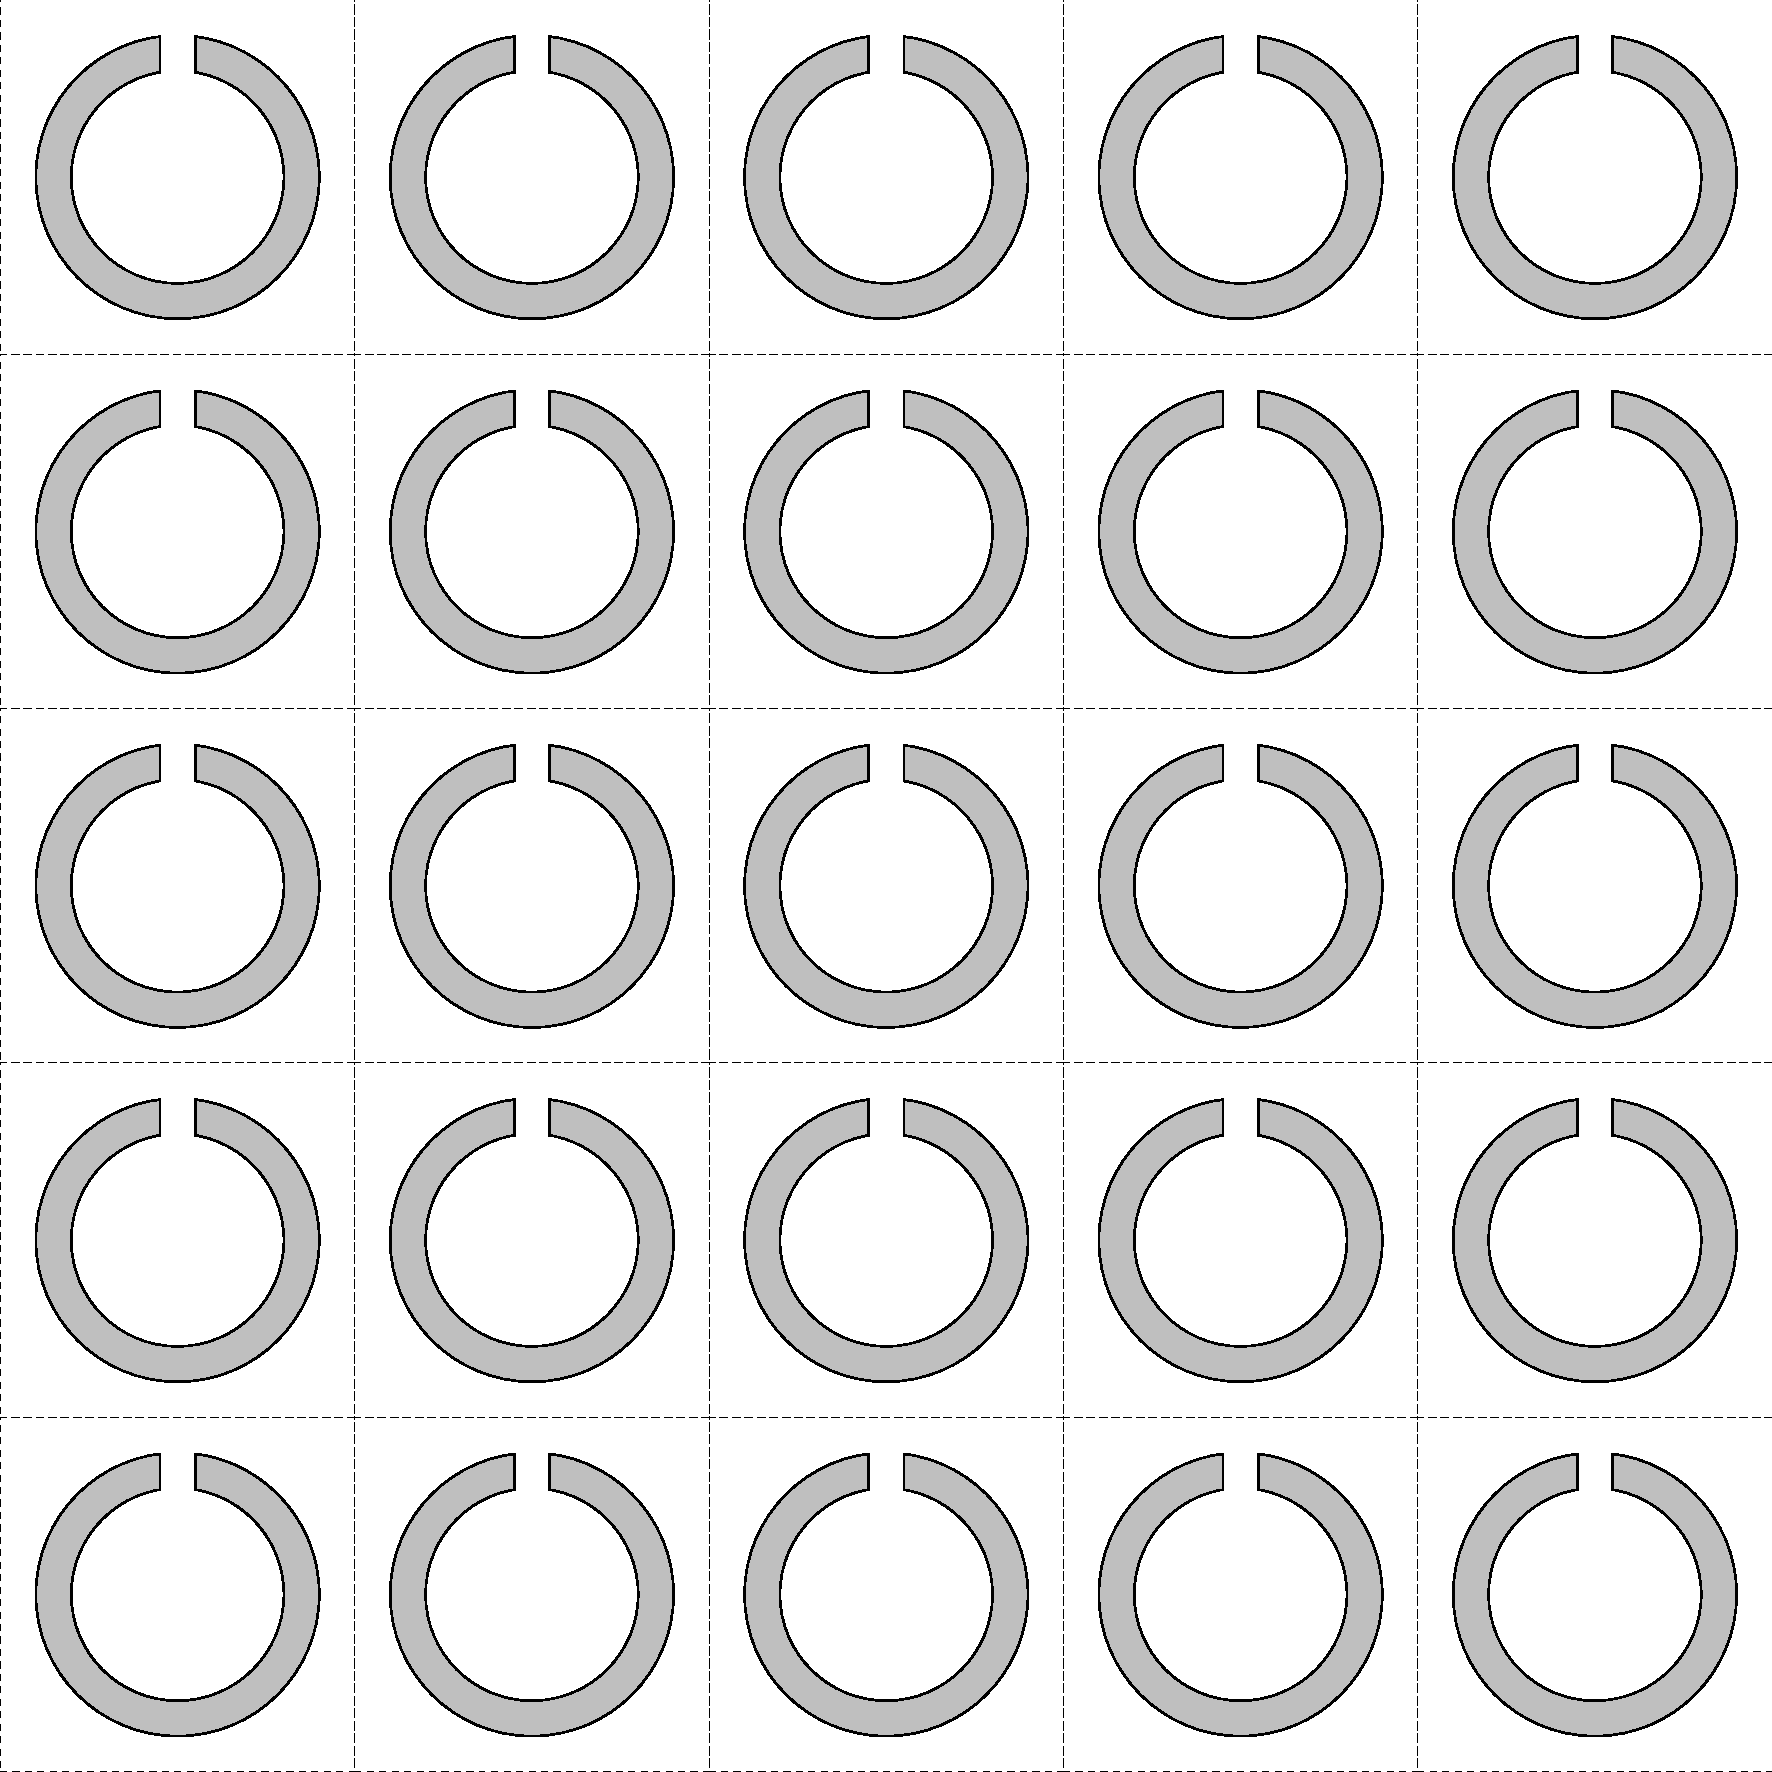
\includegraphics[width=0.8\textwidth]{Figures/SSR_structure.pdf}
            \caption{Split-ring resonator structure.}
            \label{fig:SSR_structure}
        \end{figure}

        \column{0.4\textwidth}
        
        \vspace{-4mm}
        \begin{figure}
            \centering
            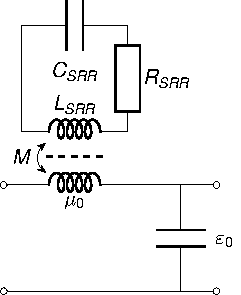
\includegraphics[width=\textwidth]{Figures/TL_negative_permeability.pdf}
            \caption{Equivalent circuit of Split-ring resonator structure.}
            \label{fig:TL_negative_permeability}
        \end{figure}
        
    \end{columns}
\end{frame}

\subsection{Double negative metamaterial}

\begin{frame}{Double negative metamaterial}
    \begin{columns}
        \column{0.5\textwidth}

        \begin{figure}
            \centering
            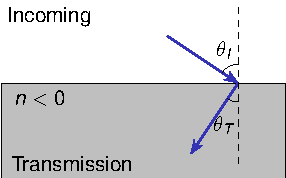
\includegraphics[width=\textwidth]{Figures/LH_Snell.pdf}
            \caption{Refraction with negative index.}
            \label{fig:LH_snell}
        \end{figure}
        \column{0.5\textwidth}
        \vspace{-8mm}
        \begin{figure}
            \centering
            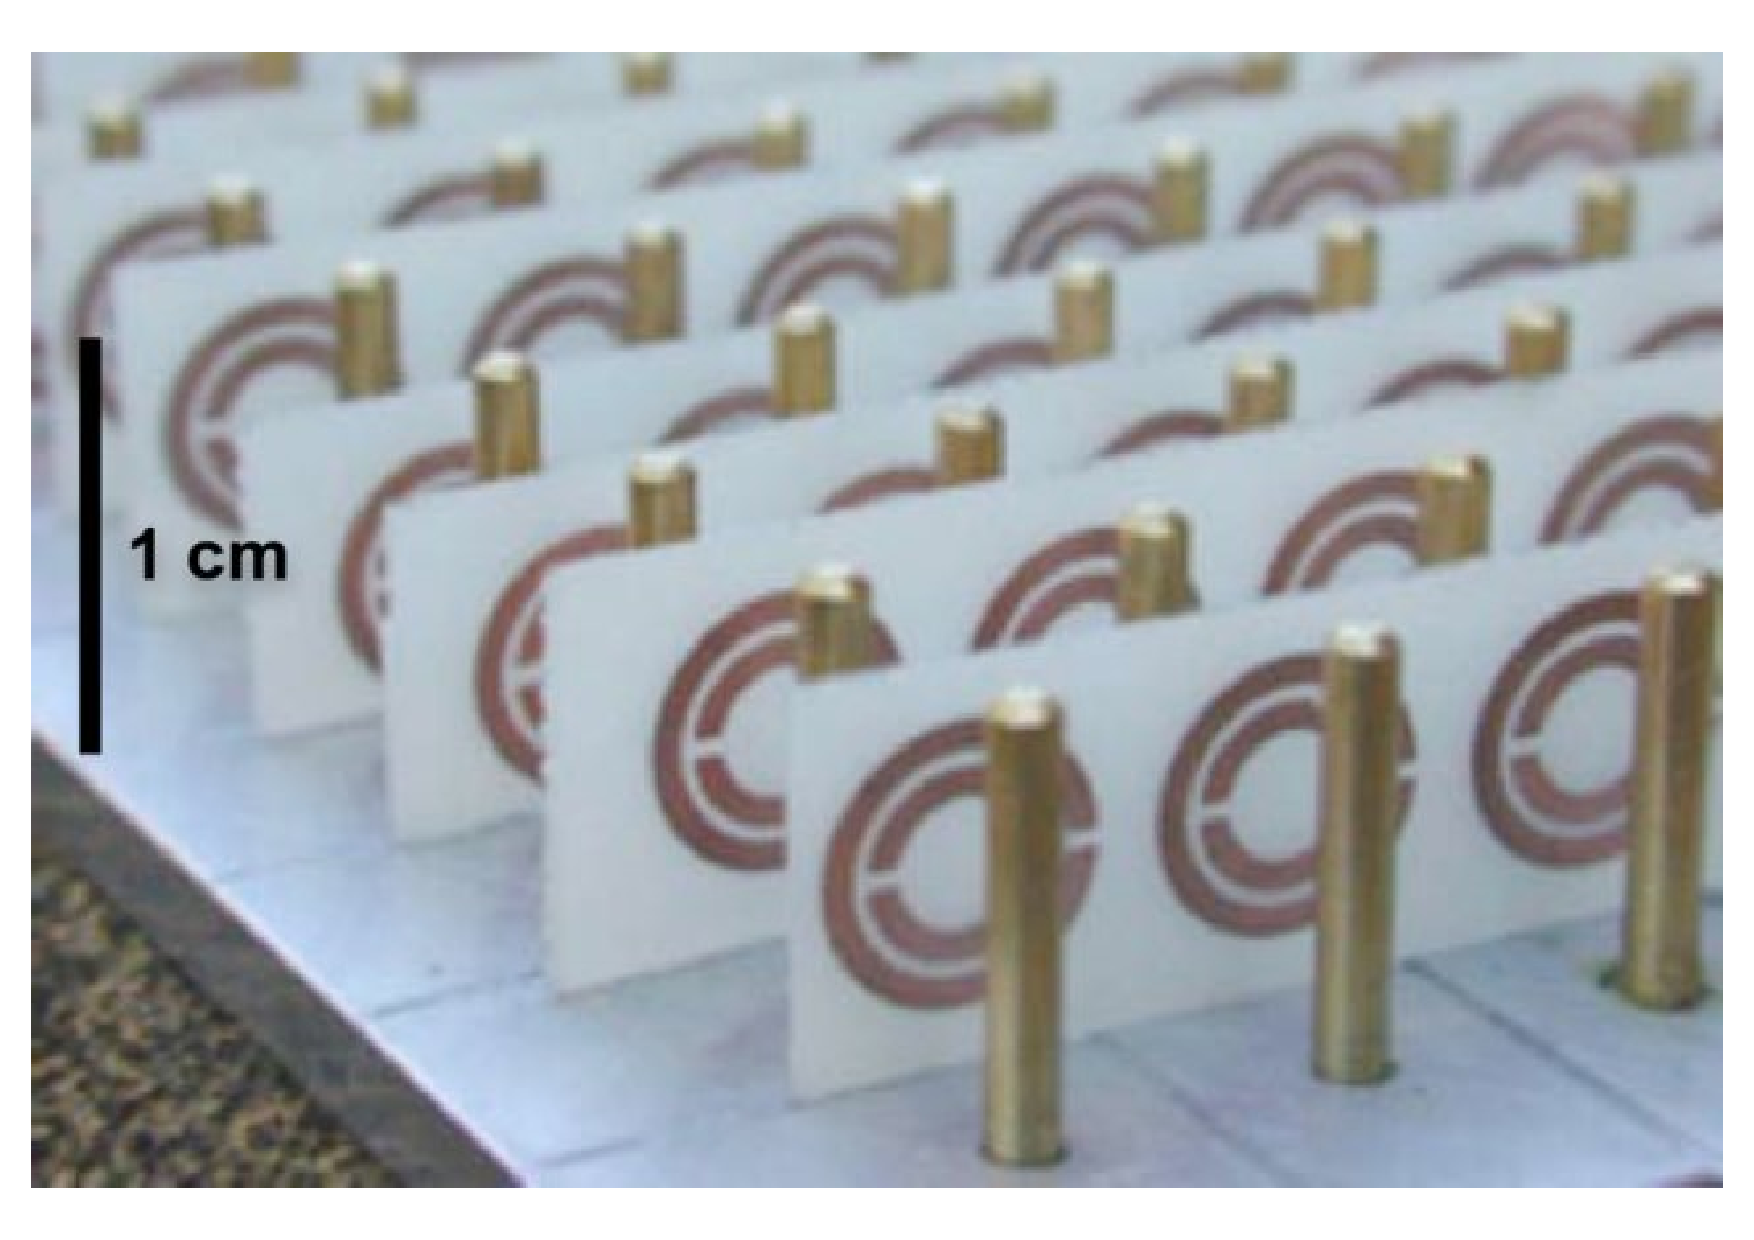
\includegraphics[width=\textwidth]{Figures/Negative_index.pdf}
            \caption{Negative refractive index metamaterial for microwaves. \cite{Ung}}
            \label{fig:Negative_index}
        \end{figure}
        \vspace{-8mm}
        \begin{figure}
            \centering
            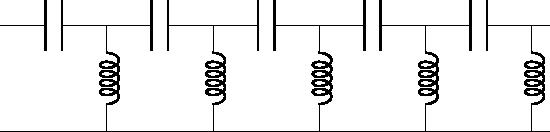
\includegraphics[width=\textwidth]{Figures/LHMM.pdf}
            \caption{Equivalent transmission line of negative index.}
            \label{fig:TL_LHMM}
        \end{figure}
        
    \end{columns}   
\end{frame}

\subsection{Superlens}

\begin{frame}{Superlens}
    \begin{figure}
        \centering
        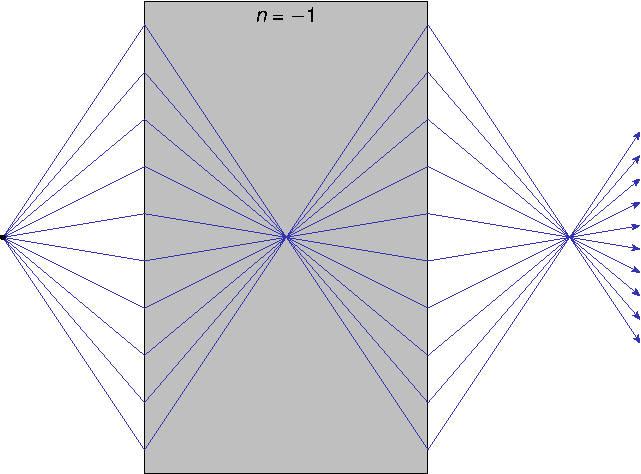
\includegraphics[width=0.8\textwidth]{Figures/LH_superlens.pdf}
        \caption{Superlens based on negative index.}
        \label{fig:LH_superlens}
    \end{figure}
    
\end{frame}

\section{Cut-wire pairs structures}

\subsection{Simple rectangle structure}

\begin{frame}{Simple rectangle struture}
    \begin{columns}
        \column{0.5\textwidth}
        \begin{itemize}
            \item Magnetic resonance frequency \cite{Zhou:06}:
        \end{itemize}
        \begin{equation*}
            f_m = \dfrac{1}{2\pi \sqrt{c_1 \varepsilon/2}} \dfrac{c_0}{l},
        \end{equation*}
        where \( 0.2 < c_1 <0.3\).
        \column{0.5\textwidth}
        \begin{figure}
            \centering
            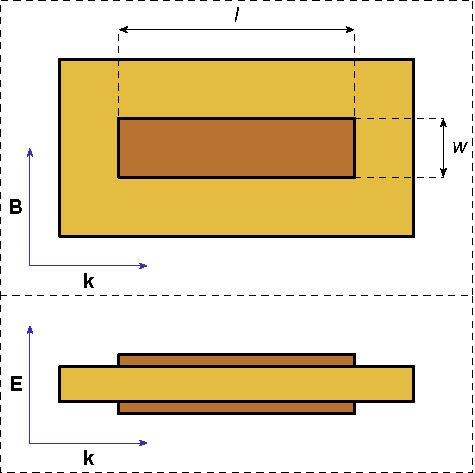
\includegraphics[width=\textwidth]{Figures/Rectangle_CWP_unitcell.pdf}
            \caption{Rectangle CWP unitcell}
            \label{fig:Rectangle_CWP_unitcell}
        \end{figure}
    \end{columns}
\end{frame}

\subsection{Cross structure}

\begin{frame}{CWP Cross structure for absorbing}
    \begin{columns}
        \column{0.5\textwidth}
        
        \begin{figure}
            \centering
            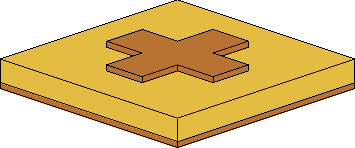
\includegraphics[width=0.9\textwidth]{Figures/3D_Meta.pdf}
            \caption{Metamaterial unitcell.}
            \label{fig:Meta_unitcell}
        \end{figure}

        \begin{itemize}
            \item Tuning leght of cross to choose resonance frequency.
            \item Tuning width of rectangle in the cross to match impedance.
        \end{itemize}
        
        \column{0.5\textwidth}
        
        \begin{figure}
            \centering
            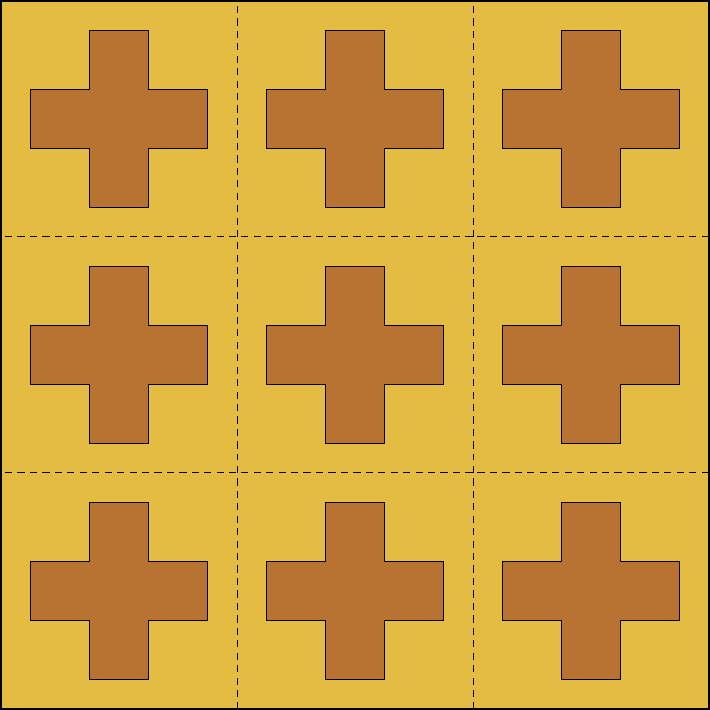
\includegraphics[width=0.9\textwidth]{Figures/Meta_full_structure.pdf}
            \caption{Cross structure.}
            \label{fig:Meta_cross_full_structure}
        \end{figure}
    \end{columns}
\end{frame}


\begin{frame}[allowframebreaks]{bibliography}

\printbibliography

\end{frame}



\end{document}
